\documentclass[11pt]{article}
\usepackage{graphicx} % This lets you include figures
\usepackage{hyperref} % This lets you make links to web locations
\usepackage[margin=0.5in]{geometry}
\usepackage[rightcaption]{sidecap}
\usepackage{subcaption}
\usepackage{wrapfig}
\usepackage{float}
\usepackage{imakeidx}
\usepackage{indentfirst}
\makeindex
%---------------------------Do Not Edit Anything Above This Line!!------------------------

% edit the line below, if needed, to change the directory name for your image files.
\graphicspath{ {./images/} }



\begin{document}

%---------------------------Edit Content in the Box to Create the Title Page--------------
\begin{titlepage}
   \begin{center}
       \vspace*{1cm}
	   \Huge
       \textbf{Project Title}

       \vspace{0.5cm}
       \Large
       Sprint Number \\
       Date \\
   \end{center}

       \vspace{1.5cm}

\begin{table}[h!]
\centering
\begin{tabular}{|l|l|}
\hline
\textbf{Name} & \textbf{Email Address} \\ \hline
Aaron Downing         & aaron.downing652@topper.wku.edu         \\ \hline
Ryerson Brower         & ryerson.brower178@topper.wku.edu         \\ \hline
Kaden Hunt         & email kaden.hunt144@topper.wku.edu         \\ \hline
\end{tabular}
\end{table}

%Latex Table Generator    
%https://www.tablesgenerator.com/     
        
\vspace{4in}

\centering        
CS 360 \\
Fall 2025\\
Project Organization Documentation

\end{titlepage}
%---------------------------Edit Content in the Box to Create the Title Page--------------


% No text here.


%---------------------------Do Not Edit Anything In This Box!!------------------------
%Table of contents and list of figures will be autogenerated by this section.
\newpage
\setcounter{page}{1}%
\cleardoublepage
\pagenumbering{gobble}
\tableofcontents
\cleardoublepage
\pagenumbering{arabic}
\clearpage
\newpage
\setcounter{page}{1}%
\cleardoublepage
\pagenumbering{gobble}
\listoffigures
\cleardoublepage
\pagenumbering{arabic}
\newpage
%---------------------------Do Not Edit Anything In This Box!!------------------------

% No text here.


%---------------------------Project Team's Organizational Approach------------------------------
\section{Project Team's Organizational Approach} %\section{} is used to create major section headers
%100 words for each sprint
	Sprint 1: %How/where did the group meet?  How often did you meet as an entire team?  Who’s the Project Manager for this sprint?
	
	Sprint 2: %How/where did the group meet?  How often did you meet as an entire team?  Who’s the Project Manager for this sprint?

	Sprint 3: %How/where did the group meet?  How often did you meet as an entire team?  Who’s the Project Manager for this sprint?

	Sprint 4: %How/where did the group meet?  How often did you meet as an entire team?  Who’s the Project Manager for this sprint?



%---------------------------End Project Team's Organizational Approach------------------------------


% No text here.


%---------------------------Schedule Organization---------------------------------------------------
\section{Schedule Organization}
%Gantt charts cover the tasks/time commitments and estimations for the entire project.  We will have four iterations of the Gantt Chart, with iteration focusing on a specific sprint.

\subsection{Gantt Chart v1:}
%100 words to describe the focus for this sprint.
%Identify the location for the Gantt Chart created during Sprint 1.  Should be clearly labeled in the project directory.
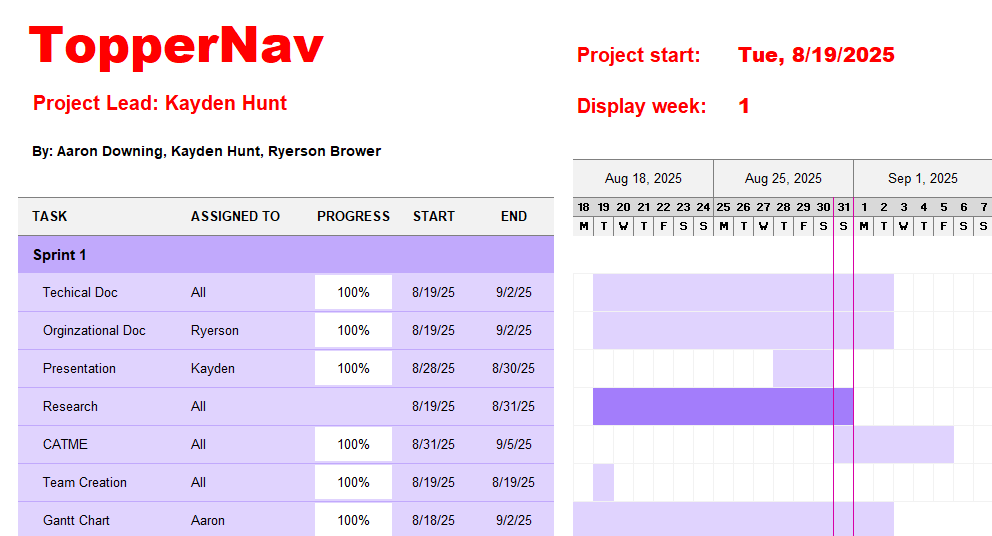
\includegraphics[scale=0.7]{TopperNavGanttChartSprint1.png} 



\subsection{Gantt Chart v2:}
%100 words to describe the focus for this sprint.
%Identify the location for the Gantt Chart created during Sprint 2.  Should be clearly labeled in the project directory.
Text goes here.



\subsection{Gantt Chart v3:}
%100 words to describe the focus for this sprint.
%Identify the location for the Gantt Chart created during Sprint 3.  Should be clearly labeled in the project directory.
Text goes here.



\subsection{Final Gantt Chart:}
%100 words to describe the focus for this sprint.
%Identify the location for the Gantt Chart created during Sprint 4.  Should be clearly labeled in the project directory.
Text goes here.



%---------------------------End Schedule Organization---------------------------------------------------


% No text here.


%---------------------------Progress Visibility---------------------------------------------------
\section{Progress Visibility}
%100 words for each sprint.
%For each sprint, explain how each member of the group is progressing with assigned tasks and how that progress is shared with the group.  Also, explain how the group is progressing with assigned tasks and how that progress is shared with the client.  Examples:  how does the group assign tasks?  How to group members know tasks assigned to them?  How do group members communicate when assigned tasks are complete, need assistance, or waiting on other tasks to be completed first?
\subsection{Sprint 1 Progress Visibility}
Text goes here.

\subsection{Sprint 2 Progress Visibility}
Text goes here.

\subsection{Sprint 3 Progress Visibility}
Text goes here.

\subsection{Sprint 4 Progress Visibility}
Text goes here.

%---------------------------End Progress Visibility---------------------------------------------------

% No text here.


%---------------------------Software Process Model---------------------------------------------------
\section{Software Process Model}
%150 words
%Describe in this section the Software Process Model used and how it increases the quality of the final deliverables.  The team should also define the quality control steps that are used in the Software Process Model.
Text goes here.

%---------------------------End Software Process Model---------------------------------------------------

% No text here.


%---------------------------Risk Management--------------------------------------------------------------
\section{Risk Management}
%Use this section to describe the team's approach to risk management.

\subsection{Risk Identification}
%List, categorize, and prioritize all potential risks associated with the project.
The following risks are listed and categorized by potential risk level.

\begin{itemize}
    \item \textbf{Database Performance (High Priority):} The database may become too slow under heavy loads, affecting responsiveness and user experience.
    \item \textbf{Route Generation API Failure (High Priority):} The external route generation API may not function as expected, preventing key functionality of the application.
    \item \textbf{Compatibility Issues (Medium Priority):} The system may encounter compatibility problems across different devices, operating systems, or software versions.
    \item \textbf{Access to Android Phones (Medium Priority):} Limited availability of Android devices for testing may hinder progress.
    \item \textbf{Large File Download (Low Priority):} Users may face issues when downloading or uploading large files, leading to performance bottlenecks.
\end{itemize}

\subsection{Risk Planning}
%Give overviews of plans for specific risk types
The team has outlined the following plans for risk planning:

\begin{itemize}
     \item \textbf{Database Performance:} Implement query optimization, proper indexing, and caching strategies. Load testing will be performed early to identify bottlenecks.
    \item \textbf{Route Generation API Failure:} Identify and test backup APIs during early development. 
    \item \textbf{Compatibility Issues:} Use emulators and virtual machines to ensure broader compatibility across various platforms.
    \item \textbf{Access to Android Phones:} Gain access to an android phone temporarily and share them among team members as needed. 
    \item \textbf{Large File Download:} Implement file compression. Clearly communicate file size limitations to users.
\end{itemize}

\subsection{Risk Monitoring}
%Give overviews of how the team will monitor specific types of risks
The following monitoring strategies will be used for the remaining duration of the project:

\begin{itemize}
    \item \textbf{Database Performance:} Monitor query execution times and system performance.
    \item \textbf{Route Generation API Failure:} Implement automated alerts for API failures or unusual latency.
    \item \textbf{Compatibility Issues:} Maintain a compatibility checklist and update it with each system change.
    \item \textbf{Access to Android Phones:} Track device usage and availability within the team. .
    \item \textbf{Large File Download:} Monitor client feedback related to file transfers.
\end{itemize}


%---------------------------Risk Management--------------------------------------------------------------





%example image:  uncomment to show usage
%\begin{figure}[h]
%    \centering
%    \includegraphics[width=1\textwidth]{images/Add_non-music.png}
%    \caption{This is how you add non-music items.}
%    \label{fig16}
%\end{figure}


%example links:  uncomment to show usage.
%\url{https://www.youtube.com}
%\href{https://www.wku.edu/}{WKU Homepage}
%\footnote{You can put the link in a footnote like this.}

% Anything to the right of a percent sign will be ignored by LaTeX.
% You can use this to put notes to yourself.  



\end{document}
